\subsection{Lightcurve}

Time series data and analyses are a fundamental aspect of solar physics 
for which many data sources are available. 
In recognition of this fact, SunPy provides a \texttt{LightCurve} object 
designed to provide a convenient and consistent interface for handling 
solar time series data. 
The main engine behind the \texttt{LightCurve} object is the \texttt{pandas} 
data analysis library. 
This library contains a large amount of functionality for manipulating 
and analysing time series data, making it an ideal basis for 
\texttt{LightCurve}.  
Like all other SunPy objects, \texttt{LightCurve} is a wrapper around 
a data object, which in this case is the \texttt{pandas} object. 

Currently, the \texttt{LightCurve} object is compatible with the following 
data sources: the GOES X-ray Sensor (XRS), PROBA2/LYRA, 
and the SDO EUV Variability Experiment (EVE). 
For each of these instruments, a sub-class of the \texttt{LightCurve} object 
is initialised (e.g. \texttt{GOESLightCurve, LYRALightCurve}) which inherits 
from \texttt{LightCurve} but allows instrument-specific functionality to be 
included. 
Future developments will introduce support for additional instruments and data 
products. 
Since time series data is generally relatively small and there is no 
established standard as to how it should be stored and distributed, 
each SunPy \texttt{LightCurve} object provides the ability to download 
its own data in its constructor.

%\subsubsection{Creating and using Lightcurves}

A \texttt{LightCurve} object may be created using a range of different methods. 
Firstly, a \texttt{LightCurve} may be created for a specific instrument based 
on an input time range. In Listing \ref{code:goes_lc_code}, 
the LightCurve constructor searches remote sites for the GOES X-ray data 
specified by the time interval, downloads the required files and subsequently 
creates the object.

\begin{listing}[H]
\begin{minted}[bgcolor=bg]{pycon}
>>> from sunpy import lightcurve
>>> goes=lightcurve.GOESLightCurve.create('2011-06-07 06:00',
...                                       '2011-06-07 08:00')
>>> goes.peek()
\end{minted}
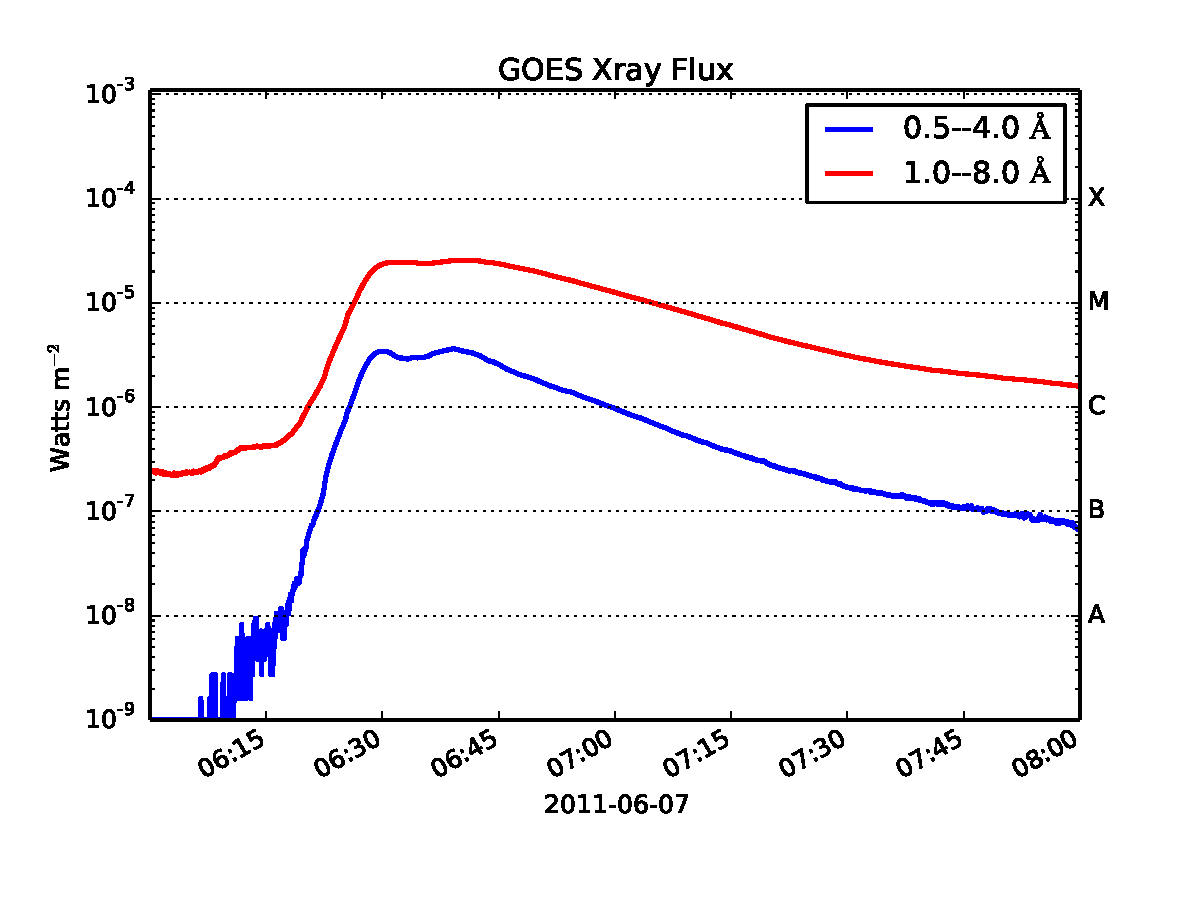
\includegraphics[width=14cm]{goes_lightcurve.pdf}
\caption{Creating a GOES lightcurve for the time interval 06:00 - 08:00 UT on 
2011 June 7 using a time range, and the result of the \texttt{peek()} method.}
\label{code:goes_lc}
\end{listing}

Alternatively, if the data file already exists on the local system, the 
\texttt{Lightcurve} object may instead be initialised using that file as input 
(see Listing \ref{code:lyra_lc}).

\begin{listing}[H]
\begin{minted}[bgcolor=bg]{pycon}
>>> from sunpy import lightcurve
>>> file='lyra_20110607-000000_lev2_std.fits'
>>> lyra=lightcurve.LYRALightCurve.create(file)
>>> lyra.peek()
\end{minted}
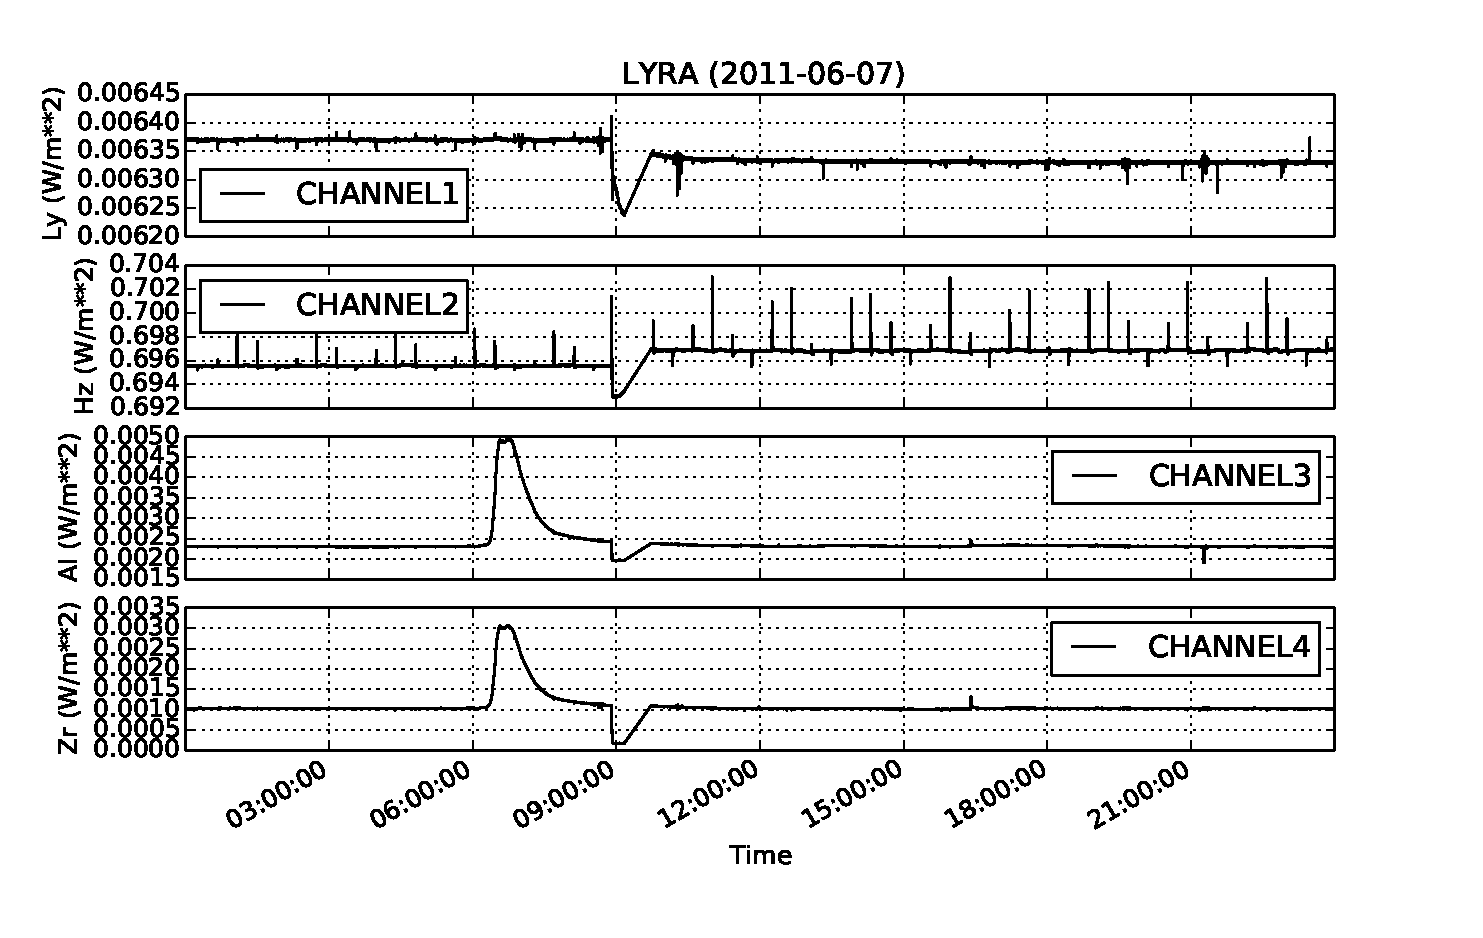
\includegraphics[width=14cm]{lyra_lightcurve.pdf}
\caption{Creating a LYRA lightcurve for the full day of 2011 June 7 using an 
existing data file, and the result of the \texttt{peek()} method}
\label{code:lyra_lc}
\end{listing}

Once the \texttt{Lightcurve} has been created it may be manipulated in 
a variety of ways in order to perform time series analysis. 
Continuing from Listing~\ref{code:lyra_lc}, we show a few simple 
examples of using a LYRA lightcurve. 

In Listing~\ref{code:lyra_lc} we created a LYRA Lightcurve spanning the 
full day of 2011 June 7. 
To extract the sub-interval 06:00 - 07:00 UT into a new \texttt{Lightcurve} 
called \texttt{lyra\_zoom} we simply do as shown on 
Listing~\ref{code:lyra_truncate}.

\begin{listing}[H]
\begin{minted}[bgcolor=bg]{pycon}
>>> from sunpy.time import TimeRange
>>> trange=TimeRange('2011-06-07 06:00','2011-06-07 07:00')
>>> lyra_zoom = lyra.truncate(trange)
\end{minted}
\caption{Extracting a sub-interval from a Lightcurve.}
\label{code:lyra_truncate}
\end{listing}

Also from the example shown in Listing~\ref{code:lyra_lc}, direct access to 
the data and time information in the object is available through 
\texttt{lyra.data} and \texttt{lyra.data.index} respectively 
(see Listing~\ref{code:lyra_pandas}).

\begin{listing}[H]
\begin{minted}[bgcolor=bg]{{pycon}
>>> print lyra.data
<class pandas.core.frame.DataFrame>
DatetimeIndex: 1496629 entries, 2011-01-28 00:00:00.110000 to 
2011-01-28 23:59:59.983993
Data columns (total 4 columns):
CHANNEL1    1496629  non-null values
CHANNEL2    1496629  non-null values
CHANNEL3    1496629  non-null values
CHANNEL4    1496629  non-null values
dtypes: float64(4)

>>> print lyra.data.index
<class pandas.tseries.index.DatetimeIndex>
[2011-01-28 00:00:00.110000, ..., 2011-01-28 23:59:59.983993]
Length: 1496629, Freq: None, Timezone: None
\end{minted}
\caption{Accessing the data and time axis in a Lightcurve}
\label{code:lyra_pandas}
\end{listing}

